\documentclass[main.tex]{subfiles}

\begin{document}
\chapter{Results}

\section{Parallelisation of self-consistent calculations of electronic-structure properties}

\subsection{First scaling tests}

The first step in analysing the scaling of \QE is to perform a baseline scaling test without any optimisations yet appplied. 
In Fig. \ref{fig:scaling_ompi_nprocs} two scaling tests on the earlier mentioned benchmarking systems Si and TaS2 are pictured. 
The \QE version used is compiled using OpenMPI 4.1.0 \todo{What exactly? Which compiler?}, without any further compilation or runtime optimisation parameters used.

\begin{figure}[htbp]
\begin{subfigure}[b]{0.3\textwidth}
    \centering
    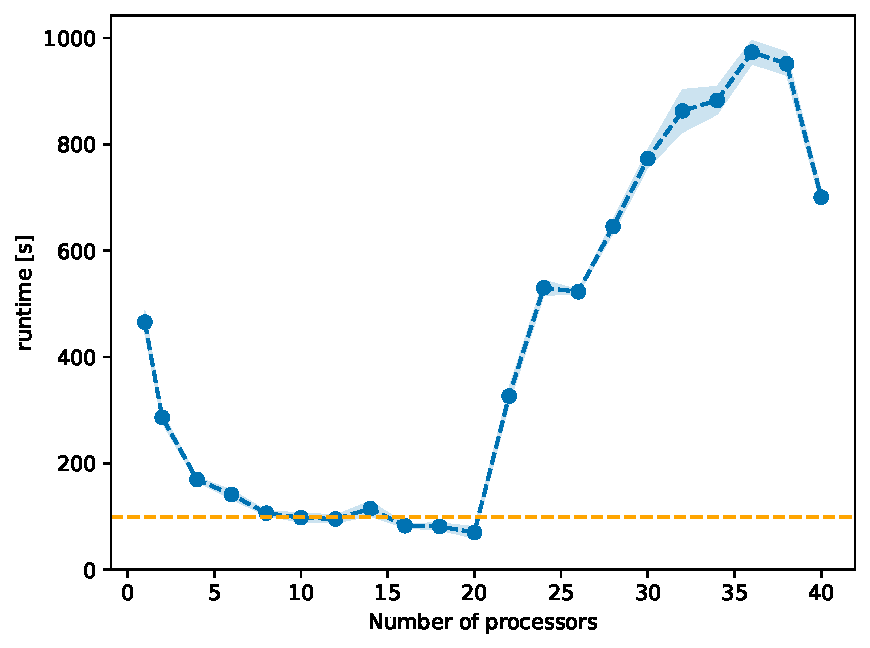
\includegraphics[width=\textwidth]{plots_scf/si_ompi_bench_nprocs_absolute.pdf}
\end{subfigure}
\begin{subfigure}[b]{0.3\textwidth}
    \centering
    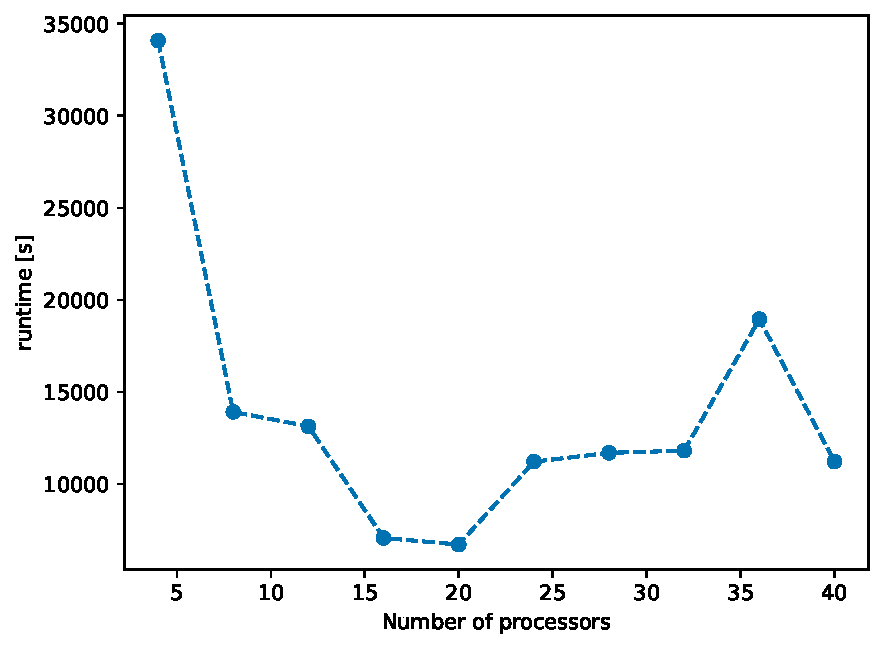
\includegraphics[width=\textwidth]{plots_scf/TaS2_ompi_bench_nprocs_absolute.pdf}
\end{subfigure}
\begin{subfigure}[b]{0.3\textwidth}
    \centering
    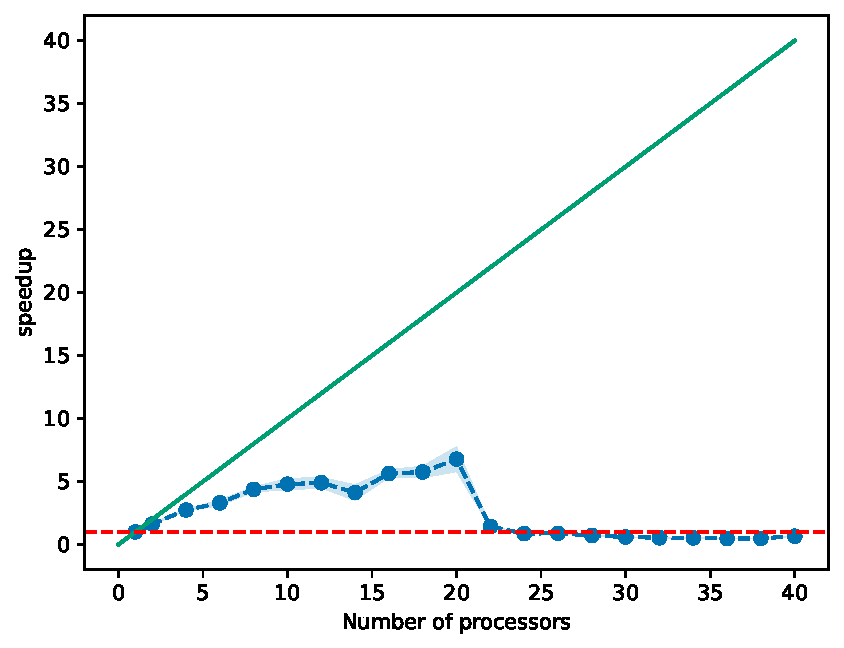
\includegraphics[width=\textwidth]{plots_scf/si_ompi_bench_nprocs_speedup.pdf}
\end{subfigure}
\begin{subfigure}[b]{0.3\textwidth}
    \centering
    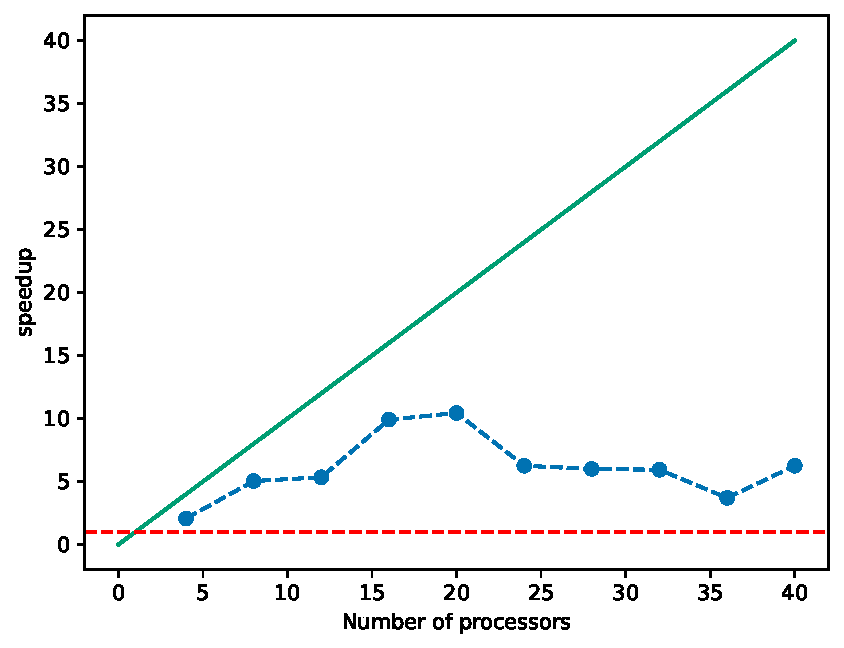
\includegraphics[width=\textwidth]{plots_scf/TaS2_ompi_bench_nprocs_speedup.pdf}
\end{subfigure}
\begin{subfigure}[b]{0.3\textwidth}
    \centering
    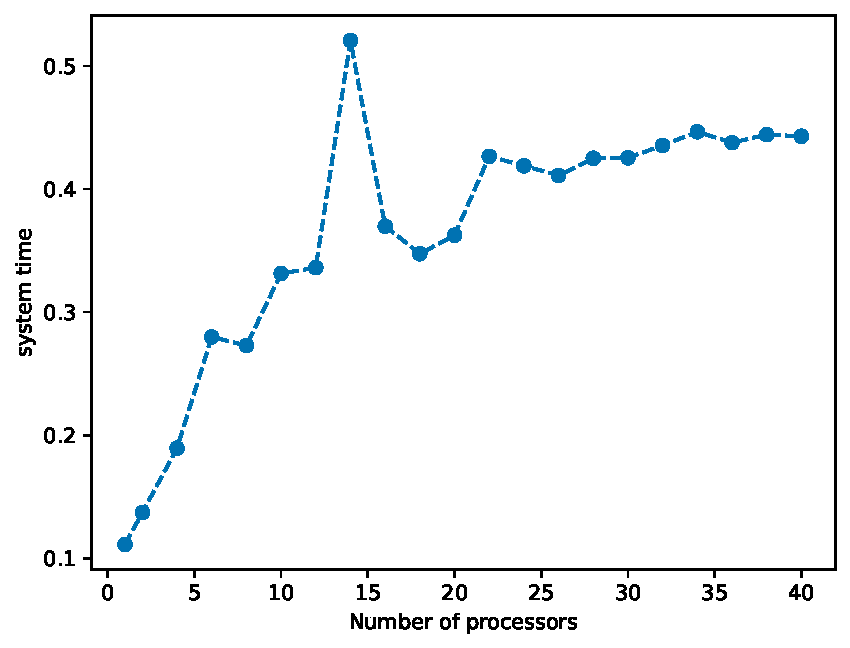
\includegraphics[width=\textwidth]{plots_scf/si_ompi_bench_nprocs_wait.pdf}
\end{subfigure}
\begin{subfigure}[b]{0.3\textwidth}
    \centering
    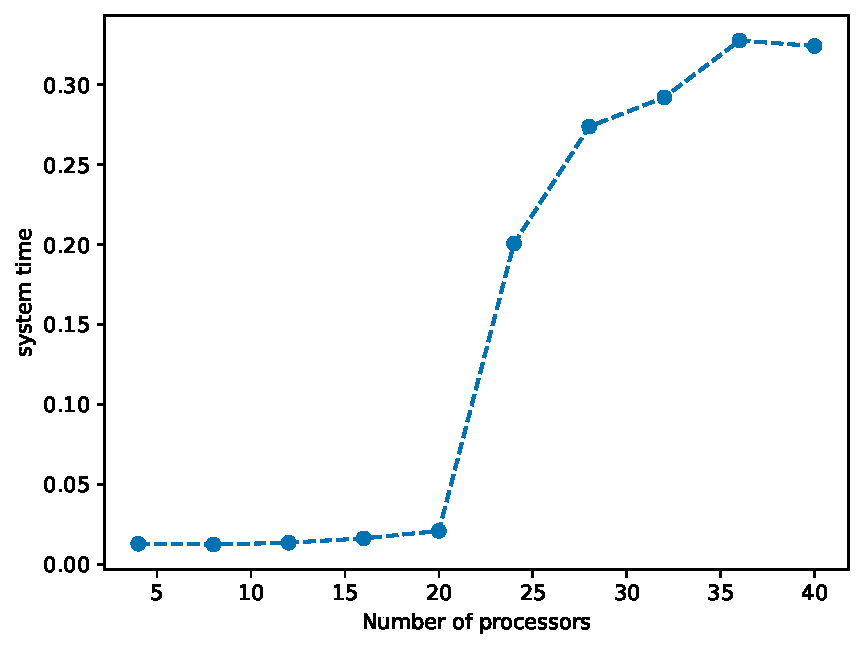
\includegraphics[width=\textwidth]{plots_scf/TaS2_ompi_bench_nprocs_wait.pdf}
\end{subfigure}
\caption{XXX}
\label{fig:scaling_ompi_nprocs}
\end{figure}

\todo{caption}

Three different metrics of scalability are pictured in \ref{fig:scaling_ompi_nprocs}.
\begin{itemize}
    \item runtime: absolute runtime of the compute job
    \item speedup: runtime divided by runtime of the job on a single core
    \item system time: percentage of wall time used by system tasks, e.g. writing to disk, etc.
\end{itemize}
For further analysis mainly speedup will be used as a metric of scalability, because it lends itself to easy interpretation: optimal scalability is achieved when the speedup scales linearly with the number of processors (with a slope of one), as discussed in ch. \ref{sec:parallel_computing}.

On a single node, both the Si and TaS2 calculations show good, but not perfect scaling behavior: the speedup does approximately scale linearly with the number of processors, but the slope is round about \(\frac{1}{2}\).
Even though the scaling behavior is not perfect, there is just a small, almost constant amount of runtime used by system calls, this speaks for good parallelisation: as discussed in ch. \ref{sec:parallel_computing}, startup time is part of every \todo{missing}

When using more than one node, not only does the scaling get worse, the execution needs longer than on a single core for the Si system, with a marginally better performance for the TaS2 system.
This is also seen in the plots of system time. The percentage of time used for tasks not directly related to calculations (mostly exchange of data in this case, which induces long waiting time when the connection between processors is not as fast as on one motherboard) goes from a near constant value for under 20 processors to 50\% of the execution time for the Si system and 35\% for the TaS2 system.

These scaling tests pose now two questions to be answered:
\begin{itemize}
    \item Is better scaling on a single node possible?
    \item How can scaling over more than one node be achieved?
\end{itemize}

\subsection{Testing different compilers and mathematical libraries}

A first strategy for solving issues with parallelization is trying different compilers and mathematical libraries.
In the PHYSnet cluster a variety of software packages is available.
For the compilation of \QE a 

For testing \QE will be compiled using the following software combinations:
\begin{itemize}
    \item OpenMPI 4.1.0 and OpenBLAS
    \item OpenMPI 4.1.0 and Scalapack
    \item Intel oneAPI 2021.4
\end{itemize}

\begin{figure}[htbp]
\begin{subfigure}[b]{0.4\textwidth}
    \centering
    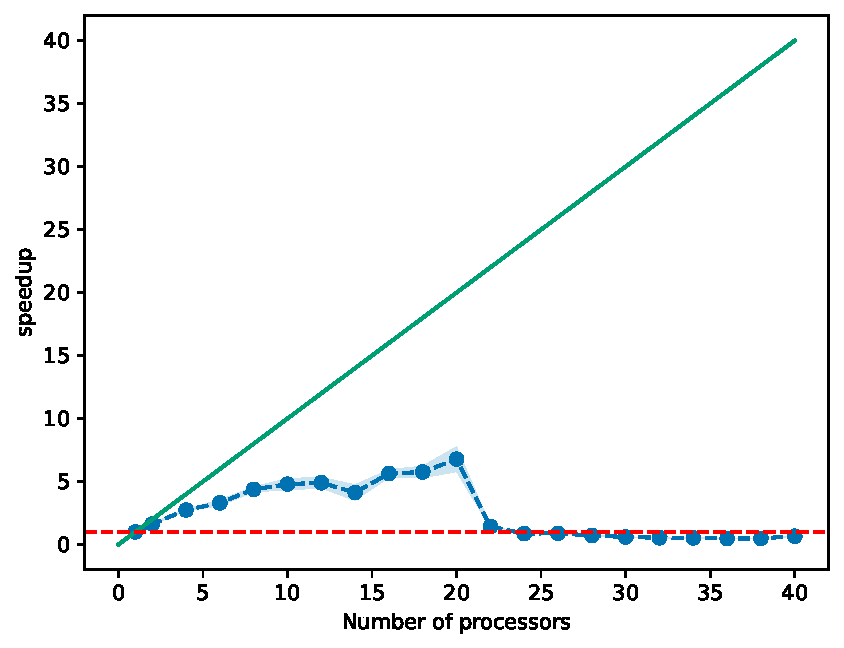
\includegraphics[width=\textwidth]{plots_scf/si_ompi_bench_nprocs_speedup.pdf}
\end{subfigure}
\begin{subfigure}[b]{0.4\textwidth}
    \centering
    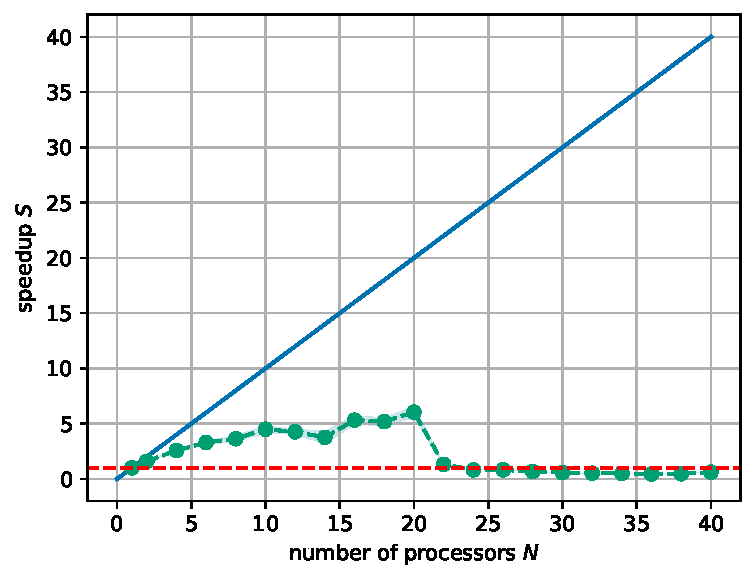
\includegraphics[width=\textwidth]{plots_scf/si_openblas_bench_nprocs_speedup.pdf}
\end{subfigure}
\begin{subfigure}[b]{0.4\textwidth}
    \centering
    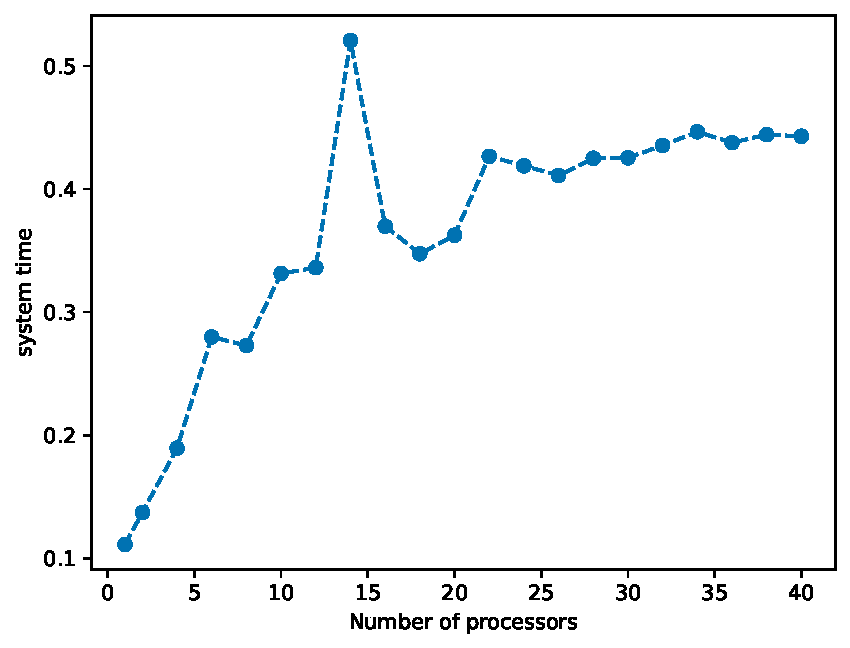
\includegraphics[width=\textwidth]{plots_scf/si_ompi_bench_nprocs_wait.pdf}
\end{subfigure}
\begin{subfigure}[b]{0.4\textwidth}
    \centering
    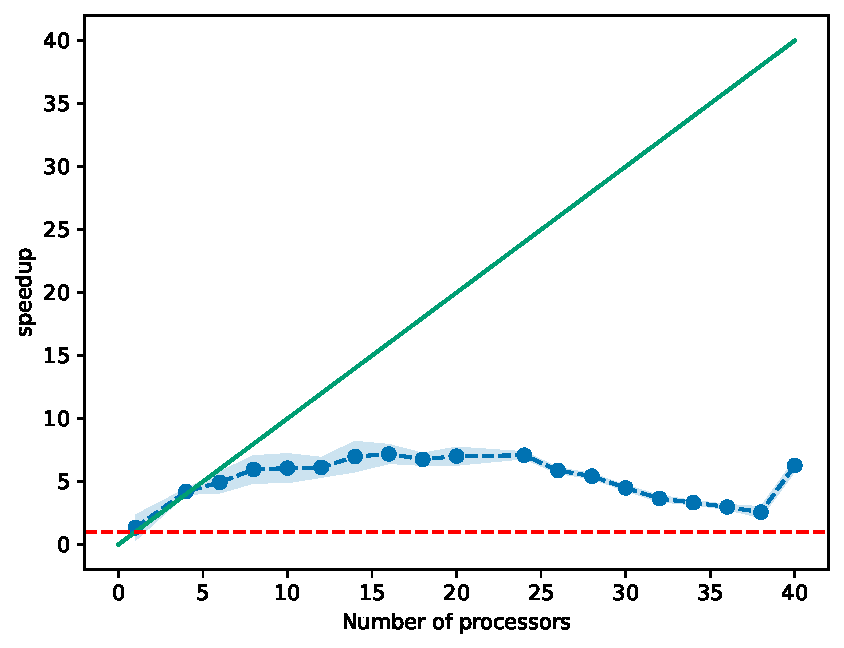
\includegraphics[width=\textwidth]{plots_scf/si_intel_bench_nprocs_speedup.pdf}
\end{subfigure}
\caption{XXX}
\label{fig:scaling_compilers_nprocs}
\end{figure}

\todo{caption}

\subsection{Using the parallelisation parameters of \QE}

As detailed in section \ref{sec:qe}, \QE offers ways to manage how the workload is distributed among the processors.
In \texttt{pw.x} k-point-parallelization and linear-algebra parallelisation are implemented.

\subsection{Comparison with calculations on the HLRN cluster}

\subsection{Scaling over 40 processors}

\subsection{Conclusion: Parameters for optimal scaling}

\end{document}